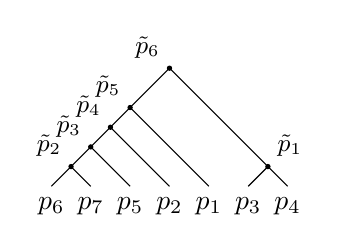
\begin{tikzpicture}[scale=1]
  \draw (0,0) -- (1.5,1.5);
  \draw (0.25,0.25) -- (0.5,0);
  \draw (0.5,0.5) -- (1,0);
  \draw (0.75,0.75) -- (1.5,0);
  \draw (1,1) -- (2,0);
  \draw (1.5,1.5) -- (3,0);
  \draw (2.75,0.25) -- (2.5,0);

  \filldraw[black] (0.25,0.25) circle (0.75pt) node[anchor=south east]{\small $\tilde{p}_{2}$};
  \filldraw[black] (0.5,0.5) circle (0.75pt) node[anchor=south east]{\small $\tilde{p}_{3}$};
  \filldraw[black] (0.75,0.75) circle (0.75pt) node[anchor=south east]{\small $\tilde{p}_{4}$};
  \filldraw[black] (1,1) circle (0.75pt) node[anchor=south east]{\small $\tilde{p}_{5}$};
  \filldraw[black] (1.5,1.5) circle (0.75pt) node[anchor=south east]{\small $\tilde{p}_{6}$};
  \filldraw[black] (2.75,0.25) circle (0.75pt) node[anchor=south west]{\small $\tilde{p}_{1}$};
  
  \draw[black] (0,-0.25) node{$p_6$};
  \draw[black] (0.5,-0.25) node{$p_7$};
  \draw[black] (1,-0.25) node{$p_5$};
  \draw[black] (1.5,-0.25) node{$p_2$};
  \draw[black] (2,-0.25) node{$p_1$};
  \draw[black] (2.5,-0.25) node{$p_3$};
  \draw[black] (3,-0.25) node{$p_4$};
\end{tikzpicture}


%%% Local Variables:
%%% mode: latex
%%% TeX-master: "main"
%%% End:
